%% Hey, emacs(1), this is -*- mode: latex; coding: utf-8; fill-column: 79 -*-

\documentclass{beamer}
\usepackage[T2A,T1]{fontenc}
\usepackage[russian,english]{babel}
\usepackage{relsize}
\usepackage{linguex}
\usepackage[utf8]{inputenc}
\usepackage{graphicx}
\usepackage{tipa} %allows IPA symbols

\newcommand{\rus}[1]{\foreignlanguage{russian}{#1}}

\AtBeginSection[]
{
  \begin{frame}
    \frametitle{Table of Contents}
    \tableofcontents[currentsection,currentsubsection]
  \end{frame}
}

\usetheme{Montpellier}
\usecolortheme{beaver}

\title[A preliminary constraint grammar for Russian] % (optional, only for long titles)
{A preliminary constraint grammar for Russian}
%\subtitle{}
\author[Tyers, Reynolds] % (optional, for multiple authors)
{F.~Tyers \and R.~Reynolds}
\institute[UiT, The Arctic University of Norway] % (optional)
{
  Department of Languages and Linguistics\\
  UiT, The Arctic University of Norway
}
\date[NODALIDA-CG 2015] % (optional)
{Constraint Grammar - Methods, Tools and Applications (NODALIDA workshop, 2015)}
\subject{Constraint Grammar, Russian, Morphosyntactic disambiguation}

\begin{document}
\frame{\titlepage}
 
\section{Goals of the paper}

\begin{frame}
\frametitle{Goals}
%\framesubtitle{}
\begin{itemize}
	\item Preliminary work on morphosyntactic disambiguator for Russian
	\pause
	\item Tuned to be high recall at the expense of precision
	\pause
	\item Evaluation
	\begin{itemize}
		\item Qualitative
		\item Task-based (word stress placement)
		\item Combining CG with HMM tagger
	\end{itemize}
\end{itemize}
\end{frame}

\section{Ambiguity in Russian} %ROB

\begin{frame}
\frametitle{Ambiguity in Russian}
\framesubtitle{}
\begin{itemize}
	\item Russian is characterized by fusional morphology
	\begin{itemize}
		\item Nouns: 12+ paradigm cells (6 main cases, sg and pl)
		\item Modifiers: 34+ paradigm cells (6 cases, 3 genders, etc.)
		\item Verbs: 13+ paradigm cells (4 past, 6 non-past, imperatives, etc.)
		% 200+ if you count participles

		\item \rus{выпей} \emph{vypej} `drink.IMP' or `bittern.Pl-GEN'
	\end{itemize}
\end{itemize}
\end{frame}

\begin{frame}
\frametitle{Three kinds of ambiguity}
\framesubtitle{}
\begin{itemize}
	\item We identify three kinds of ambiguity
	\begin{itemize}
		\item Intraparadigmatic (same lemma, different morphosyntax)
		\item Morphosyntactically incongruent (different lemma, different morphosyntax)		
		\item Morphosyntactically congruent (different lemma, same morphosyntax)
	\end{itemize}
\end{itemize}
\end{frame}

\begin{frame}
\frametitle{Intraparadigmatic ambiguity}
\framesubtitle{}
\begin{itemize}
	\item \rus{тела} \emph{tela} `body'
	\begin{itemize}
		\item \rus{т\'{е}ла} \emph{téla} SG-GEN
		\item \rus{тел\'{а}} \emph{telá} PL-NOM or PL-ACC
	\end{itemize}
	\pause
	\item \rus{новой} \emph{novoj} `new'
	\begin{itemize}
		\item ADJ-SG-FEM-GEN
		\item ADJ-SG-FEM-LOC
		\item ADJ-SG-FEM-DAT
		\item ADJ-SG-FEM-INS
	\end{itemize}
	\pause
	\item \rus{пойдём} \emph{pojdëm} `go'
	\begin{itemize}
		\item FUT-1PL `we will go'
		\item IMP-1PL `let's go!'
	\end{itemize}
\end{itemize}
\end{frame}

\begin{frame}
\frametitle{Morphysyntactically incongruent ambiguity}
\framesubtitle{}
\begin{itemize}
	\item \rus{нашей} \emph{našej}
	\begin{itemize}
		\item \rus{н\'{а}шей} \emph{nášej} `our.F-SG-GEN/DAT/LOC/INS'
		\item \rus{наш\'{е}й} \emph{našéj} `sew on.IMP-2SG'
	\end{itemize}
	\pause
	\item \rus{дорога} \emph{doroga}
	\begin{itemize}
		\item \rus{дор\'{о}га} \emph{doróga} `road.N-F-SG-NOM'
    	\item \rus{дорог\'{а}} \emph{dorogá} `dear.ADJ-F-SG-PRED'
	\end{itemize}
\end{itemize}
\end{frame}

\begin{frame}
\frametitle{Morphysyntactically congruent ambiguity}
\framesubtitle{}
\begin{itemize}
	\item \rus{замок} \emph{zamok}
	\begin{itemize}
		\item \rus{з\'{a}мок} \emph{z\'{a}mok} `castle.SG-NOM'\\
			  \rus{зам\'{о}к} \emph{zam\'{o}k} `lock.SG-NOM'
		\item \rus{з\'{a}мков} \emph{z\'{a}mkov} `castle.PL-GEN'\\
			  \rus{замк\'{о}в} \emph{zamk\'{o}v} `lock.PL-GEN'
		\item etc.
	\end{itemize}
\end{itemize}
\end{frame}

\begin{frame}
\frametitle{Frequency of each kind of ambiguity}
\framesubtitle{}
\begin{table}
  \centering
  \begin{tabular}{l|rr}
    \hline
    \textbf{Type}  & \textbf{all tokens} & \textbf{ambig. tokens} \\
    \hline
    Intraparadigm. & 59.0\%                   & 90.9\%   \\
    Incongruent    & 27.7\%                   & 42.7\%   \\ 
    Congruent      & 1.2\%                   & 1.8\%    \\ 
    \hline
  \end{tabular}
  \caption{Frequency of different types of morphosyntactic ambiguity in unrestricted text}
  %TODO caption says 'Table :' without a number
  \label{table:ambiguity}
\end{table}
\begin{itemize}
	\item \rus{з\'{a}мков} \emph{zámkov} `castle.PL-GEN'
	\item \rus{замк\'{о}в} \emph{zamkóv} `lock.PL-GEN'
	\item \rus{з\'{а}мков} \emph{zámkov} `having to do with castles.A-MSC-SG-PRED'
\end{itemize}
\end{frame}

\section{Finite-state transducer for Russian part-of-speech tagging} %ROB

\begin{frame}
\frametitle{New finite-state transducer for Russian morphological analysis}
\framesubtitle{}
\begin{itemize}
	\item We developed a finite-state transducer using the two-level formalism \cite{Koskenniemi-84}
	\begin{itemize}
		\item lexc/twolc, can be compiled in xfst or hfst
		\item analyze and generate Russian wordforms, with or without stress marks
		\pause
	\end{itemize}
	\item Based on Zaliznjak's \emph{Grammatical dictionary of Russian} \cite{Zaliznjak-77}
	\begin{itemize}
		\item includes the proper noun appendix from 2001 version
		\item supplemented with \emph{Grammatical dictionary of new Russian words} [Grishina \& Lyashevskaya 2008]
		\pause
	\end{itemize}
	\item Example output:
	\begin{itemize}
		\item \rus{новый}\texttt{{\small <adj><m><nn><sg><nom>}}\\
	    `new'
		\item \rus{автомат}\texttt{{\small <n><m><nn><sg><nom>}}\\
	    `automaton, sub-machine gun'
	\end{itemize}
\end{itemize}
\end{frame}

\section{Constraint Grammar disambiguation rules} %FRAN

\begin{frame}
\frametitle{CG rules: distribution of rule across levels}
\framesubtitle{}
\begin{table}
  \centering
  \begin{tabular}{lrrr}
    \hline
                     & {\sc select} & {\sc remove} & {\sc map} \\
    \hline
    Safe             &   16         &   34         &  -- \\
    Safe heuristic   &   89         &   76         &  -- \\
    Heuristic        &   26         &   52         &  -- \\
    Syntax labelling & --           & --           & 6 \\ 
    \hline
  \end{tabular}
  \caption{The 299 rules in the grammar are separated into four sections depending
      on rule reliability. }
  \label{tab:ruleDist}
\end{table}
\begin{itemize}
	\item Safe: real constraints in the language\\
		{\small Ex: preposition cannot directly precede a finite verb}
		\pause
	\item Safe heuristic: highly reliable tendencies\\ % Russian word order is very free
		{\small Ex: remove GEN from sentence-init. if no verb governing GEN.}
		\pause
	\item Heuristic: tendencies that are true most of the time\\ % better replaced with machine-learning
		{\small Ex: \rus{такая} is `such.FEM-SG-NOM', not `say~\rus{так}.V-PRS-ACT-ADV'}
\end{itemize}
\end{frame}


\section{Development process} %FRAN

\begin{frame}
\frametitle{Writing rules and level assignment}
\framesubtitle{}
\begin{itemize}
	\item No hand-annotated corpus was compatible with our analyser
	\pause
	\item We sorted new rules using Russian Wikipedia by collecting 100 example applications of the rule
	\pause
	\begin{itemize}
		\item Safe: 100\% correct
		\item Safe heuristic: > 97\% correct
		\item Heuristic (or discard): $\leq$ 97\% correct 
	\end{itemize}
\end{itemize}
\end{frame}

\section{Evaluation}
\subsection{Qualitative evaluation} %FRAN
\begin{frame}
\frametitle{}
\framesubtitle{}
\begin{itemize}
	\item 
	\pause
	\item 
	\begin{itemize}
		\item 
		\pause
	\end{itemize}
	\item 
\end{itemize}
\end{frame}

\subsection{Task-based evaluation} %ROB

\begin{frame}
\frametitle{Automatic word stress placement}
\framesubtitle{}
\begin{itemize}
	\item Russian word stress placement...
	\begin{itemize}
		\item ...includes complex patterns of shifting stress
		\pause
		\item ...is critical for language learners and text-to-speech\\
		\begin{itemize}
			\item \rus{догов\'{о}ром} \emph{dogovórom} > /\textipa{d@g2vOr@m}/
		\end{itemize}
		\pause
		\item ...is lexically specified: there are no universal rules of stress pattern assignment
		\pause
	\end{itemize}
	\item >7.48\% of tokens in Russian running text are stress-ambiguous
	\item Theoretically, almost 99\% of stress ambiguity can be resolved using a constraint grammar
\end{itemize}
\end{frame}

\begin{frame}
\frametitle{Automatic word stress placement - results}
\framesubtitle{}
\begin{table}
  \centering
  \begin{tabular}{r | r r r }
     & accuracy\% & error\% & abstention\%  \\
    \hline
    \hline
    {\small {\tt RussianGram}} & 90.09 & 0.79 & 9.12 \\
    {\small {\tt no CG}} & 90.07 & 0.49 & 9.44  \\
    {\small {\tt CG}} & 93.21 & 0.74 & 6.05
  \end{tabular}
  \caption{Results of stress placement task evaluation}
  \label{tab:results}
\end{table}
\begin{itemize}
	\item CG makes gains of 3.14\% (42\% of ambiguity from FST)
	\pause
	\item CG's high recall leads to a low error rate
	\pause
	\item To be continued.... (tomorrow)
\end{itemize}
\end{frame}


\subsection{Combining with HMM tagger} %FRAN

\begin{frame}
\frametitle{Combining CG with HMM tagger}
\framesubtitle{}
\begin{itemize}
	\item CG removes less than half of ambiguity
	\pause
	\item To resolve remaining ambiguity, we backoff to HMM tagger
	\begin{itemize}
		\item This approach has been applied with...\\
		Basque \cite{ezeiza.ea-98},\\
		Czech \cite{hajic.ea-01,hajic.ea-07},\\
		Norwegian \cite{johannessen.ea-11,johannessen.ea-12},\\
		Spanish \cite{hulden12},\\
		and Turkish \cite{oflazer.tur-96}
		\pause
	\end{itemize}
	\item We follow the voting method used by \cite{hulden12}
\end{itemize}
\end{frame}

\begin{frame}
\frametitle{Voting setup}
\framesubtitle{}
\begin{itemize}
	\item Freely available hunpos tagger
	\pause
	\item 10-fold cross-validation (90\% training, 10\% testing)
	\pause
	\item 3 configurations
	\begin{itemize}
		\item HMM - hunpos with default options
		\pause
		\item HMM+Morph - incorporating FST output as full-form lexicon
		\pause
		\item HMM+Morph vs CG - Voting setup: if constraint grammar left 1 valid reading,
		take that. Otherwise, take output of HMM+Morph.
	\end{itemize}
	\item 
\end{itemize}
\end{frame}

\begin{frame}
\frametitle{Voting results}
\framesubtitle{}
\begin{figure}
  \centering
  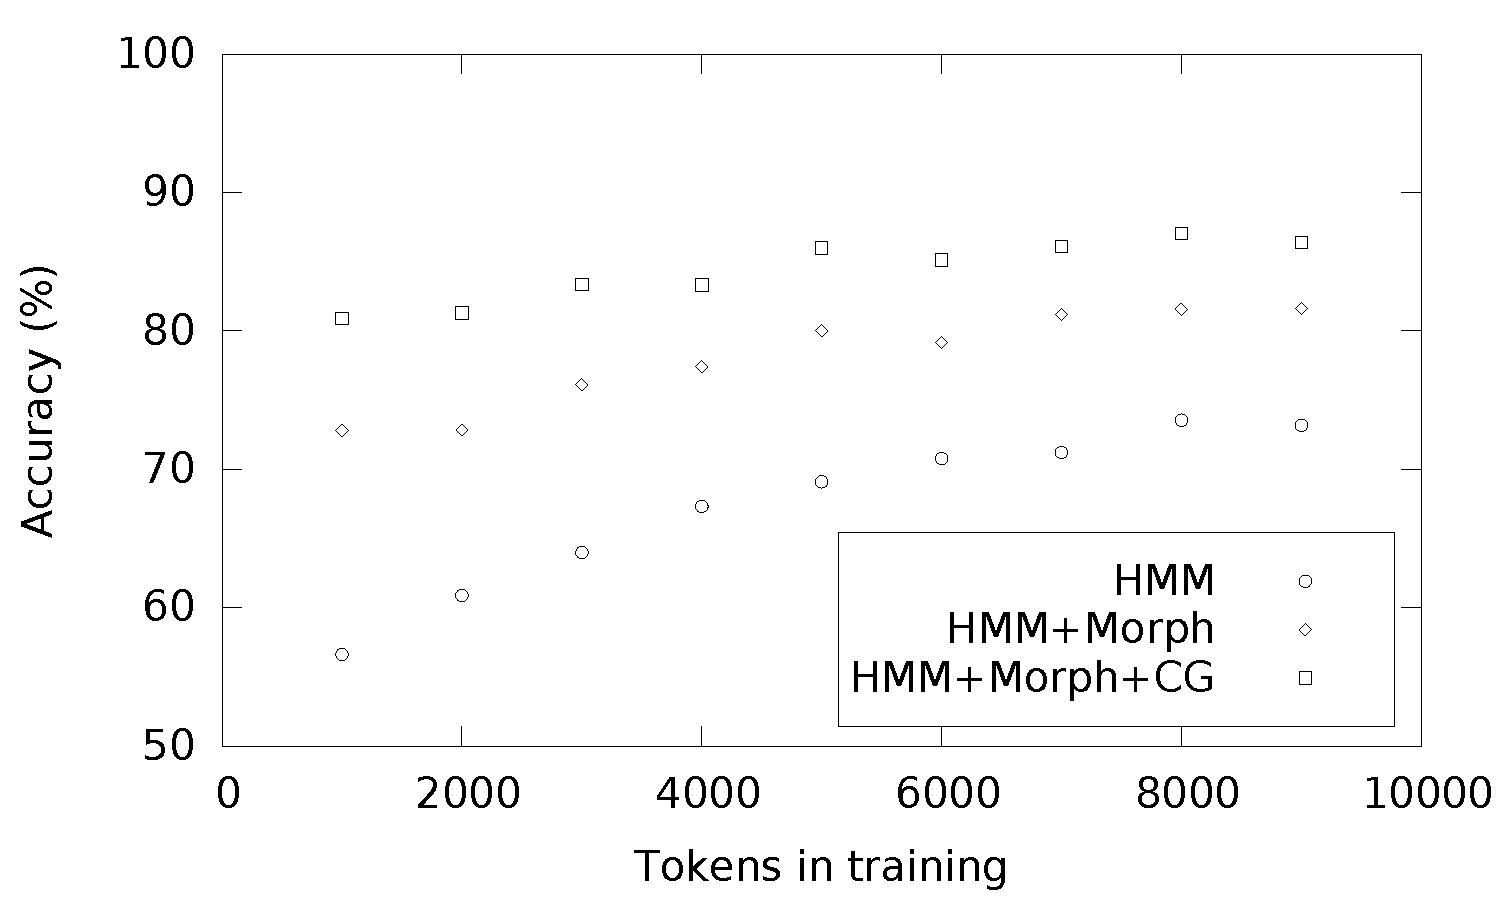
\includegraphics[width=0.70\textwidth]{graphics/learning-curve.pdf}
  %\caption{Learning curve for three taggers, \texttt{hunpos} with no lexicon, 
  %  \texttt{hunpos} with a lexicon, and \texttt{hunpos} with a lexicon and the 
  %  Russian constraint grammar in a voting set up.}
  \label{fig:curve}
\end{figure}
\begin{itemize}
	\item hunpos tagger alone is more dependent on training-corpus size
	\pause
	\item 
	\pause
	\item 
	\item 
\end{itemize}
\end{frame}


\section{Future work and conclusions} %FRAN

\begin{frame}
\frametitle{Future work}
\framesubtitle{}
\begin{itemize}
	\item Improve precision while maintaining high recall
	\pause
	\item Add syntactic functions and dependency parsing
	\begin{itemize}
		\item We plan to use Giellatekno's dependency parser \cite{antonsen10}
		\pause
	\end{itemize}
	\item Improve workflow by extending our gold-standard corpus while checking new rule accuracy
\end{itemize}
\end{frame}

\begin{frame}
\frametitle{Conclusions}
\framesubtitle{}
\begin{itemize}
	\item Preliminary constraint grammar for Russian
	\pause
	\begin{itemize}
		\item Tuned for high recall at expense of precision
		\pause
		\item Rules are assigned to levels, based on tested accuracy
		\pause
		\item Improves performance of trigram HMM-based tagger
		\pause
	\end{itemize}
	\item Improve workflow by extending our gold-standard corpus while checking new rule accuracy
\end{itemize}
\end{frame}

\bibliographystyle{apalike}
\begin{tiny}
\bibliography{ruscg}
\end{tiny}
\end{document}
